% Created 2017-01-02 Mon 14:43
% Intended LaTeX compiler: pdflatex
\documentclass{article}
\usepackage[utf8]{inputenc}
\usepackage[T1]{fontenc}
\usepackage{graphicx}
\usepackage{grffile}
\usepackage{longtable}
\usepackage{wrapfig}
\usepackage{rotating}
\usepackage[normalem]{ulem}
\usepackage{amsmath}
\usepackage{textcomp}
\usepackage{amssymb}
\usepackage{capt-of}
\usepackage{hyperref}
\usepackage[a4paper, total={7in, 10in}]{geometry}
\usepackage[utf8]{inputenc}
\usepackage[english]{babel}
\usepackage{minted}
\usemintedstyle{emacs}
\renewcommand{\familydefault}{\rmdefault}
\usepackage[usenames, dvipsnames]{xcolor}
\pagenumbering{arabic}
\usepackage{hyperref}
\hypersetup{colorlinks=true, linkcolor=blue, filecolor=magenta, urlcolor=cyan}
\urlstyle{same}
\author{Sachin\thanks{psachin@redhat.com}}
\date{\today}
\title{Red Hat OpenStack Platform - Swift}
\hypersetup{
 pdfauthor={Sachin},
 pdftitle={Red Hat OpenStack Platform - Swift},
 pdfkeywords={},
 pdfsubject={},
 pdfcreator={Emacs 25.1.1 (Org mode 9.0)}, 
 pdflang={English}}
\begin{document}

\maketitle

\section{Theory}
\label{sec:orgfbdcad6}
\begin{itemize}
\item Swift allows users to store unstructured data(objects) with
canonical names containing \emph{three} part:
\begin{itemize}
\item \texttt{/account}: Think \emph{account} as a storage location and NOT user
account. \emph{account} stores meta-data of that account, plus
list of all containers in that account. \emph{account} is analogous
to \texttt{/home} directory which may holds multiple users.

\item \texttt{/account/container}: Think of container as a root directory
of user(analogous to \texttt{/home/<USER>/}). Account can have many
containers with no limit.

\item \texttt{/account/container/object}: This is actual file. User may
start storing a single file(files are stored in container as
an object), or hierarchical data like \newline
\texttt{/photos/alaska/magic-bus/me.jpg} as an object. Swift stores
multiple copies of single object across physical locations to
ensure the data reliability and availability.
\end{itemize}

\item Remember that, user do not have to know the actual location of the
data. In-fact he never knows. User always access the data in the
form of \texttt{/account/container/object}.
\end{itemize}

\section{Handy commands}
\label{sec:org9f4f928}
\begin{itemize}
\item \emph{My settings}:
\begin{itemize}
\item Swift server address: \hfill \texttt{saio:8080}
\item AuthURL: \hfill \texttt{http://saio:8080/auth/v1.0}
\item PublicURL/StorageURL: \hfill \texttt{http://saio:8080/v1/AUTH\_wasteland}
\item account: \hfill \texttt{wasteland}
\item container: \hfill \texttt{keys}
\item object: \hfill \texttt{mykey.pem}
\end{itemize}

\item If you have access to Swift server, \texttt{Pubic-URL/StorageURL},
\texttt{Auth-Token}, \& \texttt{account} can be fetched using following command,
\begin{minted}[]{sh}
swift stat -v
#                     StorageURL: http://saio:8080/v1/AUTH_wasteland
#                     Auth Token: AUTH_tk968b0ae7947640be874af6cd897a2b1e
#                        Account: AUTH_wasteland
#                     Containers: 0
#                        Objects: 0
#                          Bytes: 0
# Containers in policy "default": 1
#    Objects in policy "default": 0
#      Bytes in policy "default": 0
#                  Accept-Ranges: bytes
#                    X-Timestamp: 1463138224.81309
#                     X-Trans-Id: tx1fe3ecbeb9f04fdc92287-005735e92c
#                   Content-Type: text/plain; charset=utf-8
\end{minted}
\end{itemize}


\begin{itemize}
\item New user can be added as follows,
\begin{minted}[]{sh}
# --- /etc/swift/proxy-server.conf ---
[filter:tempauth]
use = egg:swift#tempauth
# user_ACCOUNT_USER = PASSWORD [GROUP] <storage URL:8080>
user_wasteland_psachin = psachin .admin .reseller_admin

[app:proxy-server]
use = egg:swift#proxy
allow_account_management = true
account_autocreate = true
# --- File ends here ---

# Restart servers and Proxy
swift-init account restart
swift-init container restart
swift-init object restart
swift-init proxy restart
\end{minted}
\item Managing container and object using \texttt{swift} command

Set following environmental variables
\begin{minted}[]{sh}
# --- ~/.profile ---
export ST_AUTH=http://saio:8080/auth/v1.0
export ST_USER=wasteland:psachin
export ST_KEY=psachin
# --- File ends here ---
\end{minted}

Source the file before executing any command
\begin{minted}[]{sh}
source ~/.profile
\end{minted}

\emph{Most of the time, no configuration is needed, if Swift is
enabled during packstack. You can actually start from here.}
\begin{minted}[]{sh}
# --- Create container: 'keys' ---
swift post keys
# Verify/list containers
swift list
# --- Upload an object to container ---
# Create a file
echo "746c1c636cebe7a888fd77688dbfc252" > mykey.pem
# Upload object-'mykey.pem' to container-'keys'
swift upload keys mykey.pem
# Verify the object
swift list keys
# --- Download object ---
swift download keys mykey.pem
# Download object with different name
swift download keys mykey.pem -o mykey2.pem
\end{minted}

\begin{itemize}
\item Another way to access swift container/object is to provide
username \& password.
\begin{minted}[]{sh}
# swift -U <ACCOUNT>:<USER> -K <PASSWORD> COMMAND
swift -U wasteland:psachin -K psachin stat -v
#                     StorageURL: http://saio:8080/v1/AUTH_wasteland
#                     Auth Token: AUTH_tkf551ef98eb1e442b9efcef1261d87c64
#                        Account: AUTH_wasteland
#                     Containers: 1
#                        Objects: 0
#                          Bytes: 0
# Containers in policy "default": 1
#    Objects in policy "default": 0
#      Bytes in policy "default": 0
#                  Accept-Ranges: bytes
#                    X-Timestamp: 1463292608.77517
#                     X-Trans-Id: txc8bc7ba0659b497fb170f-00573b0ff4
#                   Content-Type: text/plain; charset=utf-8

# Upload an object
# swift -U <ACCOUNT>:<USER> -K <PASSWORD> upload <CONTAINER> <file/object>
swift -U wasteland:psachin -K psachin upload keys mykey.pem
\end{minted}
\end{itemize}
\item Managing container and object using APIs(\texttt{curl} command)
\begin{minted}[]{sh}
# --- Get token ---
# Set authURL and publicURL
export authURL="http://saio:8080/auth/v1.0/"
export publicURL="http://saio:8080/v1/AUTH_wasteland"

curl -v \
	 -H "X-Auth-User: wasteland:psachin" \
	 -H "X-Auth-Key: psachin" \
	 $authURL

# *   Trying 192.168.8.80...
# * Connected to 192.168.8.80 (192.168.8.80) port 8080 (#0)
# > GET /auth/v1.0/ HTTP/1.1
# > Host: 192.168.8.80:8080
# > User-Agent: curl/7.43.0
# > Accept: */*
# > X-Auth-User: wasteland:psachin
# > X-Auth-Key: psachin
# >
# < HTTP/1.1 200 OK
# < X-Storage-Url: http://192.168.8.80:8080/v1/AUTH_wasteland
# < X-Auth-Token-Expires: 82975
# < X-Auth-Token: AUTH_tk968b0ae7947640be874af6cd897a2b1e
# < Content-Type: text/html; charset=UTF-8
# < X-Storage-Token: AUTH_tk968b0ae7947640be874af6cd897a2b1e
# < Content-Length: 0
# < X-Trans-Id: tx9c1bef9065754dd9b68ec-005735c49d
# < Date: Fri, 13 May 2016 12:12:13 GMT
# <
# * Connection #0 to host 192.168.8.80 left intact

export token="AUTH_tk968b0ae7947640be874af6cd897a2b1e"

# Verify account access
curl -v \
	 -H "X-Storage-Token: $token" \
	 $publicURL

# *   Trying 192.168.8.80...
# * Connected to 192.168.8.80 (192.168.8.80) port 8080 (#0)
# > GET /v1/AUTH_wasteland HTTP/1.1
# > Host: 192.168.8.80:8080
# > User-Agent: curl/7.43.0
# > Accept: */*
# > X-Storage-Token: AUTH_tk968b0ae7947640be874af6cd897a2b1e
# >
# < HTTP/1.1 204 No Content
# < Content-Length: 0
# < Accept-Ranges: bytes
# < X-Account-Object-Count: 0
# < X-Account-Storage-Policy-Default-Bytes-Used: 0
# < X-Account-Storage-Policy-Default-Object-Count: 0
# < X-Timestamp: 1463138224.81309
# < X-Account-Bytes-Used: 0
# < X-Account-Container-Count: 0
# < Content-Type: text/plain; charset=utf-8
# < X-Account-Storage-Policy-Default-Container-Count: 0
# < X-Trans-Id: tx95142c218202459399c88-005735cac1
# < Date: Fri, 13 May 2016 12:38:25 GMT
# <
# * Connection #0 to host 192.168.8.80 left intact

# --- Create a container: 'keys' ---
curl -v \
	 -H "X-Storage-Token: $token" \
	 -X PUT $publicURL/keys

# *   Trying 192.168.8.80...
# * Connected to 192.168.8.80 (192.168.8.80) port 8080 (#0)
# > PUT /v1/AUTH_wasteland/keys HTTP/1.1
# > Host: 192.168.8.80:8080
# > User-Agent: curl/7.43.0
# > Accept: */*
# > X-Storage-Token: AUTH_tk968b0ae7947640be874af6cd897a2b1e
# >
# < HTTP/1.1 201 Created
# < Content-Length: 0
# < Content-Type: text/html; charset=UTF-8
# < X-Trans-Id: tx39b7aee463b64127adfe2-005735cb92
# < Date: Fri, 13 May 2016 12:41:54 GMT
# <
# * Connection #0 to host 192.168.8.80 left intact

# Verify container
curl -v \
	 -H "X-Storage-Token: $token" \
	 -X GET $publicURL/keys

# *   Trying 192.168.8.80...
# * Connected to 192.168.8.80 (192.168.8.80) port 8080 (#0)
# > GET /v1/AUTH_wasteland/keys HTTP/1.1
# > Host: 192.168.8.80:8080
# > User-Agent: curl/7.43.0
# > Accept: */*
# > X-Storage-Token: AUTH_tk968b0ae7947640be874af6cd897a2b1e
# >
# < HTTP/1.1 204 No Content
# < Content-Length: 0
# < X-Container-Object-Count: 0
# < Accept-Ranges: bytes
# < X-Storage-Policy: default
# < X-Container-Bytes-Used: 0
# < X-Timestamp: 1463138224.83257
# < Content-Type: text/html; charset=UTF-8
# < X-Trans-Id: tx05408e3d41c246ea930f5-005735cc21
# < Date: Fri, 13 May 2016 12:44:17 GMT
# <
# * Connection #0 to host 192.168.8.80 left intact

# --- Upload object to container ---
# Create a file
echo "746c1c636cebe7a888fd77688dbfc252" > mykey.pem

# Upload object-'mykey.pem' to container-'keys'
curl -v \
	 -H "X-Storage-Token: $token" \
	 -X PUT $publicURL/keys/mykey.pem -T mykey.pem

# *   Trying 192.168.8.80...
# * Connected to 192.168.8.80 (192.168.8.80) port 8080 (#0)
# > PUT /v1/AUTH_wasteland/keys/mykey.pem HTTP/1.1
# > Host: 192.168.8.80:8080
# > User-Agent: curl/7.43.0
# > Accept: */*
# > X-Storage-Token: AUTH_tk968b0ae7947640be874af6cd897a2b1e
# > Content-Length: 43
# > Expect: 100-continue
# >
# < HTTP/1.1 100 Continue
# * We are completely uploaded and fine
# < HTTP/1.1 201 Created
# < Last-Modified: Fri, 13 May 2016 12:53:00 GMT
# < Content-Length: 0
# < Etag: 640ebd176639fb6ef9a3227770ee7b17
# < Content-Type: text/html; charset=UTF-8
# < X-Trans-Id: txf33923d6fbfe4523b4451-005735ce2b
# < Date: Fri, 13 May 2016 12:52:59 GMT
# <
# * Connection #0 to host 192.168.8.80 left intact

# Download an object
curl -v \
	 -H "X-Storage-Token: $token" \
	 -X GET $publicURL/keys/mykey.pem > mykey.pem

# *   Trying 192.168.8.80...
#   % Total    % Received % Xferd  Average Speed   Time    Time     Time  Current
#                                  Dload  Upload   Total   Spent    Left  Speed
	#   0     0    0     0    0     0      0      0 --:--:-- --:--:-- --:--:-- 0* \
#                          Connected to 192.168.8.80 (192.168.8.80) port 8080 (#0)
# > GET /v1/AUTH_wasteland/keys/mykey.pem HTTP/1.1
# > Host: 192.168.8.80:8080
# > User-Agent: curl/7.43.0
# > Accept: */*
# > X-Storage-Token: AUTH_tk968b0ae7947640be874af6cd897a2b1e
# >
# < HTTP/1.1 200 OK
# < Content-Length: 43
# < Accept-Ranges: bytes
# < Last-Modified: Fri, 13 May 2016 12:53:00 GMT
# < Etag: 640ebd176639fb6ef9a3227770ee7b17
# < X-Timestamp: 1463143979.89953
# < Content-Type: application/octet-stream
# < X-Trans-Id: tx6b14a272331b4bc6937db-005735cef1
# < Date: Fri, 13 May 2016 12:56:17 GMT
# <
# { [43 bytes data]
# 100    43  100    43    0     0   2748      0 --:--:-- --:--:-- --:--:--  2866
# * Connection #0 to host 192.168.8.80 left intact
\end{minted}

\item Get statistics
\begin{minted}[]{sh}
# Auth related information
swift auth
# export OS_STORAGE_URL=http://saio:8080/v1/AUTH_wasteland
# export OS_AUTH_TOKEN=AUTH_tkf551ef98eb1e442b9efcef1261d87c64

swift auth -v
# export ST_AUTH=http://saio:8080/auth/v1.0
# export ST_USER=wasteland:psachin
# export ST_KEY=psachin

# To obtain Storage URL and Auth-Token
swift stat -v

# Get statistics of container and/or object
swift stat [container]
swift stat [container] [object]

# Retrive capability of proxy
swift capabilities
# Core: swift
#  Options:
#   account_autocreate: True
#   account_listing_limit: 10000
#   allow_account_management: True
#   container_listing_limit: 10000
#   extra_header_count: 0
#   max_account_name_length: 256
#   max_container_name_length: 256
#   max_file_size: 5368709122
#   max_header_size: 8192
#   max_meta_count: 90
#   max_meta_name_length: 128
#   max_meta_overall_size: 4096
#   max_meta_value_length: 256
#   max_object_name_length: 1024
#   policies: [{u'default': True, u'name': u'default', u'aliases': u'default'}]
#   strict_cors_mode: True
#   version: 2.7.1.dev83
# Additional middleware: bulk_delete
#  Options:
#   max_deletes_per_request: 10000
#   max_failed_deletes: 1000
# Additional middleware: bulk_upload
#  Options:
#   max_containers_per_extraction: 10000
#   max_failed_extractions: 1000
# Additional middleware: container_sync
#  Options:
#   realms: {u'TEST': {u'clusters': {u'SAIO': {u'current': True}}}}
# Additional middleware: slo
#  Options:
#   max_manifest_segments: 1000
#   max_manifest_size: 2097152
#   min_segment_size: 1
# Additional middleware: staticweb
# Additional middleware: tempauth
#  Options:
#   account_acls: True
# Additional middleware: tempurl
#  Options:
#   incoming_allow_headers: []
#   incoming_remove_headers: [u'x-timestamp']
#   methods: [u'GET', u'HEAD', u'PUT', u'POST', u'DELETE']
#   outgoing_allow_headers: [u'x-object-meta-public-*']
#   outgoing_remove_headers: [u'x-object-meta-*']

# List container's details(Similar to `ls -lh`)
swift list --lh [container]
\end{minted}

\item Object versioning

When an object is overwritten, it's older version is lost, but
there is a way we can store older version(s) of an object, no
matter how many times is was overwritten.

To enable object versioning, set \texttt{allow\_versions} option to
\texttt{true} in container configuration file.
\begin{minted}[]{sh}
# --- /etc/swift/container-server.conf ---
[app:container-server]
allow_versions = true
# --- File ends here ---

# --- Create containers ---
# Create 'archive' container to hold 'current' container's object versions
swift post archive

# Now create 'current' container with header 'X-Versions-Location'
# pointing to 'archive'
swift post current -H "X-Versions-Location: archive"

# --- Other similar ways(Optional) ---
# May also define content length at the time of creating a container
swift post archive -H "content-length: 0"
swift post current -H "content-length: 0" -H "X-Versions-Location: archive"

# And also specify Read ACL(World readable) during container creation
swift post -r ".r:*" archive -H "content-length: 0"
swift post -r ".r:*" current -H "content-length: 0" -H "X-Versions-Location: archive"
# --- xxx ---
\end{minted}

\begin{itemize}
\item \url{https://www.youtube.com/watch?v=ru2iMJvUZjI}
\end{itemize}

\item Managing account quota

\begin{itemize}
\item \emph{Note: Write request to metadata entry is only permitted to
reseller.} Make sure you have \texttt{reseller\_admin} group associated
with user

\begin{minted}[]{sh}
# /etc/swift/proxy-server.conf
[filter:tempauth]
use = egg:swift#tempauth
user_admin_admin = admin .admin .reseller_admin
user_test_tester = testing .admin .reseller_admin
user_test2_tester2 = testing2 .admin
user_test_tester3 = testing3
\end{minted}

\item Set account quotas

\begin{minted}[]{sh}
# 10K bytes
swift post -m quota-bytes:13000
# OR
swift post -H "X-Account-Meta-Quota-Bytes:13000"

# 3 objects
swift post -m quota-count:3
# OR
swift post -H "X-Account-Meta-Quota-Count:3"


swift stat -v
#                  StorageURL: http://saio:8080/v1/AUTH_test
#                  Auth Token: AUTH_tk665649077fc74fca88eebd7274de17f4
#                     Account: AUTH_test
#                  Containers: 1
#                     Objects: 1
#                       Bytes: 83412
# Containers in policy "gold": 1
#    Objects in policy "gold": 1
#      Bytes in policy "gold": 83412
#            Meta Quota-Bytes: 13000
#            Meta Quota-Count: 3
#                  X-Trans-Id: tx491cefe71fa848199480c-00586a834c
#      X-Openstack-Request-Id: tx491cefe71fa848199480c-00586a834c
#                 X-Timestamp: 1483034243.85889
#                Content-Type: text/plain; charset=utf-8
#               Accept-Ranges: bytes
\end{minted}
\end{itemize}

\item Managing container's quota

\begin{minted}[]{sh}
# Limit maximum of 2 objects in container 'keys'
swift post -m quota-count:3 keys
# OR
swift post -H "X-Container-Meta-Quota-Count: 2" keys

# Max size of an object should be not more than 512 bytes in container 'keys'
swift post -m quota-count:512 keys
# OR
swift post -H "X-Container-Meta-Quota-Bytes: 512" keys

swift stat -v keys
#                    URL: http://saio:8080/v1/AUTH_test/keys
#             Auth Token: AUTH_tk665649077fc74fca88eebd7274de17f4
#                Account: AUTH_test
#              Container: keys
#                Objects: 1
#                  Bytes: 83412
#               Read ACL:
#              Write ACL:
#                Sync To:
#               Sync Key:
#       Meta Quota-Count: 3
#       Meta Quota-Bytes: 512
#          Last-Modified: Mon, 02 Jan 2017 16:42:27 GMT
#          Accept-Ranges: bytes
#       X-Storage-Policy: gold
#            X-Timestamp: 1483362272.23768
#             X-Trans-Id: tx9387af8e677745d18ffe3-00586a82fb
# X-Openstack-Request-Id: tx9387af8e677745d18ffe3-00586a82fb
#           Content-Type: text/plain; charset=utf-8
\end{minted}
\end{itemize}


\section{Builder files}
\label{sec:org54d6419}
\begin{itemize}
\item Acts as a database
\item Python pickle
\begin{minted}[linenos,firstnumber=1]{python}
import pickle
print(pickle.load(open('object.builder')))
\end{minted}
\item Ring builder command
\begin{minted}[]{sh}
# Account server runs on port 6002
swift-ring-builder add account.builder <region><zone>-<IP>:6002/<device><weight>
# Container server runs on port 6001
swift-ring-builder add container.builder <region><zone>-<IP>:6001/<device><weight>
# and the Object server runs on port 6000
swift-ring-builder add object.builder <region><zone>-<IP>:6000/<device><weight>
swift-ring-builder add object-N.builder <region><zone>-<IP>:6000/<device><weight>
\end{minted}
\item Region: Geographical location
\item Zone: within region isolation
\item Weight: Relative number of partition a drive will have
\begin{itemize}
\item 1TB \textasciitilde{} Weight of 100.0
\item 2TB \textasciitilde{} Weight of 200.0..
\end{itemize}
\end{itemize}
\section{Swift Ring}
\label{sec:org2e43154}
\begin{itemize}
\item Data structure
\item Describes your cluster
\item One ring each for \texttt{account}, \texttt{container}, \& \texttt{object}
\begin{minted}[]{sh}
# swift-ring-builder account.builder create <PartitionPower> <Replicas> <MinPartHrs>

cd /etc/swift/
swift-ring-builder account.builder create 10 3 1
swift-ring-builder container.builder create 10 3 1
swift-ring-builder object.builder create 10 3 1
\end{minted}

\item How to decide value of Partition Power?

Assume that I have a system with 4 drives right now, but the
maximum drives I can go up-to is 10.
\begin{minted}[]{sh}
# Partition Power
2^part_power > (Nos. of drives you think you will have at-scale) * 100

# I may have 10 drives in future
2^part_power > 10 * 100
2^part_power > 1000
2^10 > 1000
1024 > 1000  # 2^10 = 1024 just goes above 1000, which is perfect.
\end{minted}

\item Calculate Partition Power(Python snippet)
\begin{minted}[linenos,firstnumber=1]{python}
# Use python3 interpreter
from math import log2, ceil
print(ceil(log2(10 * 100)))  # 10 <- Partition Power
\end{minted}

\item Partition in Swift

\begin{minted}[]{sh}
/srv/2/node/sdb2/objects/171/a56/2ae7be8de859228d6575cc9fe5518a56/1479968148.23926.data

/srv/2/node/sdb2/objects/171 # partition number
/srv/2/node/sdb2/objects/171/a56 # last 3 chars from hashed objectname
/srv/2/node/sdb2/objects/171/a56/2ae7be8de859228d6575cc9fe5518a56/ # hashed objectname
/srv/2/node/sdb2/objects/171/a56/2ae7be8de859228d6575cc9fe5518a56/1479968148 # timestamp
\end{minted}

\item Swift partition table
\end{itemize}


\begin{center}
\begin{tabular}{llll}
 & Replica \# 1 & Replica \# 2 & Replica \#3\\
\hline
Partition \# 0 & Device \# 0 & Device \# 3 & Device \# 2\\
Partition \# 1 & Device \# 1 & Device \# 2 & Device \# 0\\
Partition \# 2 & Device \# 4 & Device \# 1 & Device \# 3\\
\end{tabular}
\end{center}

\begin{center}
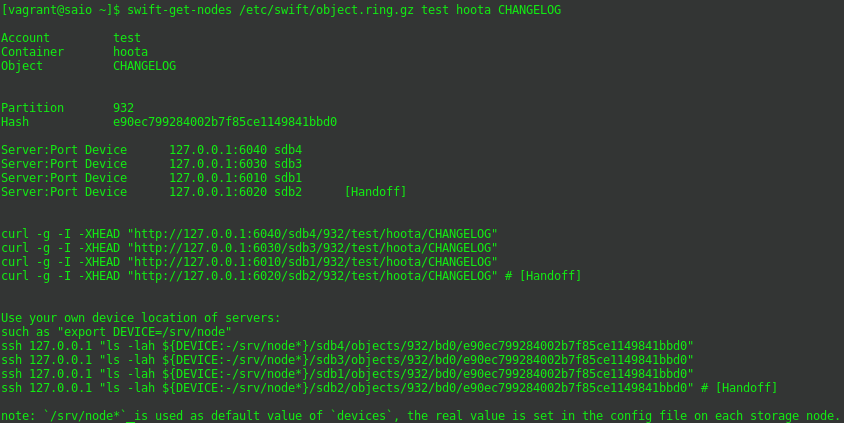
\includegraphics[width=.9\linewidth]{./swift-get-nodes.png}
\end{center}

\section{Additional notes}
\label{sec:org1dac3d4}
\emph{Swift} consistency processes:
\begin{itemize}
\item \emph{Auditor}: Will walk through the storage nodes, read the data and
the checksum, ensure the checksum matched with the database
checksum. If the checksum didn't match, the data is moved to the
Quarantine.
\item \emph{Replicator}: The replicator, will also scan each drive and
ensures that the replicas of data is stored where is supposed to
live. If it does not finds the data in that place(may be the
data, due to corruption was moved to Quarantine), it will push
the data to that place.
\end{itemize}


\begin{itemize}
\item Storage policies
\begin{itemize}
\item Decide where you want to store data
\begin{itemize}
\item Between swift clusters
\item Subset of hardware
\end{itemize}
\item Erasure coding(Data availability policies)
\begin{itemize}
\item Based in frequency of access
\item Example:
\begin{minted}[]{sh}
swift post -H "X-Storage-Policy: gold" container_gold
swift post -H "X-Storage-Policy: silver" container_silver
swift post -H "X-Storage-Policy: ec42" container_ec42

swift upload container_gold cirros-0.3.4-x86_64-disk.img
swift upload container_silver cirros-0.3.4-x86_64-disk.img
swift upload container_ec42 cirros-0.3.4-x86_64-disk.img
\end{minted}
\end{itemize}
\end{itemize}

\item Erasure Codes
\begin{itemize}
\item At the time if building a ring for Erasure codes, number of
replicas are replaced with number of fragments

\begin{minted}[]{sh}
swift-ring-builder object.builder create 10 6 1
\end{minted}

where 4 + 2 = 6

4 data fragments
2 parity data

So that the system can sustain 4 disk failures before the data is
treated to be lost

\item Erasure coding is implemented in Swift as storage policies

\begin{minted}[]{sh}
# /etc/swift/swift.conf
[storage-policy:2]
name = ec42
policy_type = erasure_coding
ec_type = liberasurecode_rs_vand
ec_num_data_fragments = 4
ec_num_parity_fragments = 2
\end{minted}

\item \url{https://www.youtube.com/watch?v=kH3DXMKlEr8}
\item \url{https://www.youtube.com/watch?v=GDNK1S4FJBQ}
\end{itemize}

\item ACLs
\begin{itemize}
\item Container ACL
\begin{minted}[]{sh}
# World readable
swift post -r ".r:*" photos

# Allow .welcome.com but deny .noisy.com
swift post -r ".r:*.welcome.com,.r:-noisy.com" photos

# Enable object listing within a container
swift post -r ".r:*,.rlistings" photos
\end{minted}
\end{itemize}

\item Hashing
\begin{itemize}
\item Swift hashing function
\begin{minted}[linenos,firstnumber=1]{python}
# Use python3 interpreter
# Swift hashing is based on MD5
# hash(path) = md5(path + per-cluster suffix)

# Python snippet to know on which drive the object will be stored,
# assuming I have 4 drives
from hashlib import md5

m = md5()
m.update("/account/container/object")  # Hypothetical path
digest = m.hexdigest()
print(digest)

# hex to int
hex2int = int(digest, 16)
print(hex2int)
# digest % (number of drives) = Drive number
print(hex2int % 4)  # 2
\end{minted}
\end{itemize}

\item Account access
\begin{itemize}
\item Using Python interpreter
\begin{minted}[]{python}
>>> import swift.common.memcached as mc
>>> mc = mc.MemcacheRing(['127.0.01:11211'])
>>> mc.get('AUTH_/user/test:tester')
u'AUTH_tk8e047f9a96cc48759319b7781ddeb992'
>>> mc.get('AUTH_/token/AUTH_tk8e047f9a96cc48759319b7781ddeb992')
[1481115804.307723, u'test,test:tester,AUTH_test']
\end{minted}

\item Shell
\begin{minted}[]{sh}
swift stat -v
#     			   StorageURL: http://saio:8080/v1/AUTH_test
#     			   Auth Token: AUTH_tk8e047f9a96cc48759319b7781ddeb992
#     				  Account: AUTH_test
#     			   Containers: 27
#     				  Objects: 22
#                         Bytes: 13328148
#   Containers in policy "ec42": 12
#      Objects in policy "ec42": 11
#        Bytes in policy "ec42": 13288056
# Containers in policy "silver": 1
#    Objects in policy "silver": 0
#      Bytes in policy "silver": 0
#   Containers in policy "gold": 14
#      Objects in policy "gold": 11
#        Bytes in policy "gold": 40092
#     			   X-Trans-Id: txb4f4f6812c514fce91f15-005846ebc6
#     			  X-Timestamp: 1480517025.85633
#                  Content-Type: text/plain; charset=utf-8
#                 Accept-Ranges: bytes
\end{minted}
\end{itemize}
\end{itemize}

\section{Object expirer}
\label{sec:org22a06d4}

\begin{itemize}
\item Start object expirer server

\begin{minted}[]{sh}
swift-init object-expirer start
\end{minted}

\item Schedule deletion of object after user deletes the file

\begin{minted}[]{sh}
swift delete container_gold cirros-0.3.4-x86_64-disk.img -H "X-Delete-After: 120"
\end{minted}
\end{itemize}

\section{Swift handoff partitions}
\label{sec:orgf0a98fe}
\begin{itemize}
\item How is a handoff partition flagged versus a partition that is
marked to be moved during a rebalance?

\emph{Answer} (notmyname): "handoff" is only a thing defined by the
results of the call to \texttt{get\_more\_nodes()}. it's not a concept
that means anything with regards to rebalancing. ie it's not
"flagged" or anything. handoffs are just an ordered walk through
the ring
\end{itemize}


\begin{itemize}
\item How should one think of handoff devices?

\emph{Answer} (mattoliverau): A hand off device is a non primary node
for a certain partition in the ring. Things are placed to hand
off nodes when either

\begin{itemize}
\item there wasn't enough primary nodes to keep it durable.
\item when write affinity has been set and you want to get your
object durability written to a closer region or zone
\item on a ring rebalance
\end{itemize}
When looking for an object (GET) swift will check all primary
nodes for the object and then some of the hand off nodes.

But in essence once on a handoff node, we have durability which
is the most important. but if the primaries are busy or down you
may not get your object back until swift corrects it self

The replicators will look at the objects they have, and if its a
partition they're a hand off for, becuase they received it cause
other primaries where down, or a rebalance suddenly has now
suddenly made them a handoff node for a partition, they will
replicate it out to the primary nodes and then if successful,
delete it.

handoff nodes + eventual consistancy helps swift keep its awesome
durability
\end{itemize}


\begin{itemize}
\item is it (handoff node) meant to be a temporary holding place?

\emph{Answer} (mattoliverau): Yeah
\end{itemize}

\section{Swift on OpenStack(RHOSP-8)}
\label{sec:orgdb9d675}

\begin{itemize}
\item undercloud

Verify swift authentication using below command

\begin{minted}[]{sh}
[stack@undercloud ~]$ source stackrc

[stack@undercloud ~]$ swift list

[stack@undercloud ~]$ swift stat -v
#      StorageURL: http://192.0.2.1:8080/v1/AUTH_447097d6f2844cdf9d5d0fa7b8529046
#      Auth Token: e117add154fc429f92fba2a00fdbaaf0
#         Account: AUTH_447097d6f2844cdf9d5d0fa7b8529046
#      Containers: 0
#         Objects: 0
#      	   Bytes: 0
# X-Put-Timestamp: 1481719100.59059
#     X-Timestamp: 1481719100.59059
#      X-Trans-Id: txd2aa20b0ed084bfc8a059-0058513d3c
#     ontent-Type: text/plain; charset=utf-8

[stack@undercloud ~]$ swift auth -v
export OS_IDENTITY_API_VERSION=2.0
export OS_AUTH_VERSION=2.0
export OS_AUTH_URL=http://192.0.2.1:5000/v2.0
export OS_PASSWORD=Redhat01
export OS_TENANT_NAME=admin
export OS_USERNAME=admin
\end{minted}

Password is derived from puppet configs

\begin{minted}[]{sh}
[stack@undercloud:/etc]# grep -r Redhat01 *
puppet/hieradata/puppet-stack-config.yaml:heat::keystone::domain::keystone_password: Redhat01
puppet/hieradata/puppet-stack-config.yaml:keystone::roles::admin::password: Redhat01
puppet/hieradata/puppet-stack-config.yaml:admin_password: Redhat01
\end{minted}

You will find IP address in \texttt{/etc/ironic/ironic.conf}

\begin{minted}[]{sh}
...
my_ip=192.0.2.1
...
\end{minted}

Access swift using \texttt{curl}

\begin{itemize}
\item Get \textbf{admin} account UUID

\begin{minted}[]{sh}
[stack@undercloud]$ openstack project list
+----------------------------------+---------+
| ID                               | Name    |
+----------------------------------+---------+
| 447097d6f2844cdf9d5d0fa7b8529046 | admin   |
| 31f55360edff4a1d81670daf65d720a2 | service |
+----------------------------------+---------+
\end{minted}

\item Get token

\begin{minted}[]{sh}
[stack@undercloud]# openstack token issue
+------------+----------------------------------+
| Field      | Value                            |
+------------+----------------------------------+
| expires    | 2016-12-14T17:05:37Z             |
| id         | 2de6e7295e1b481a9c12b264ace5284c |
| project_id | 447097d6f2844cdf9d5d0fa7b8529046 |
| user_id    | b62e1dfc83e5479db4c258b31ebb57bb |
+------------+----------------------------------+
\end{minted}

\item User admin token and UUID to access swift

\begin{minted}[]{sh}
[stack@undercloud]# curl -v -H "X-Storage-Token: 2de6e7295e1b481a9c12b264ace5284c" \
			   http://192.0.2.1:8080/v1/AUTH_447097d6f2844cdf9d5d0fa7b8529046
* About to connect() to 192.0.2.1 port 8080 (#0)
*   Trying 192.0.2.1...
* Connected to 192.0.2.1 (192.0.2.1) port 8080 (#0)
> GET /v1/AUTH_447097d6f2844cdf9d5d0fa7b8529046 HTTP/1.1
> User-Agent: curl/7.29.0
> Host: 192.0.2.1:8080
> Accept: */*
> X-Storage-Token: 2de6e7295e1b481a9c12b264ace5284c
>
< HTTP/1.1 204 No Content
< Content-Type: text/plain; charset=utf-8
< X-Account-Object-Count: 0
< X-Timestamp: 1481720818.51417
< X-Account-Bytes-Used: 0
< X-Account-Container-Count: 0
< X-Put-Timestamp: 1481720818.51417
< Content-Length: 0
< X-Trans-Id: tx2aac9d2dbbe443f3aa758-00585143f2
< Date: Wed, 14 Dec 2016 13:06:58 GMT
<
* Connection #0 to host 192.0.2.1 left intact
\end{minted}
\end{itemize}
\end{itemize}


\begin{itemize}
\item TODO: overcloud

\begin{minted}[]{sh}
[stack@undercloud ~]$ source overcloudrc
[stack@undercloud ~]$ swift auth -v
export OS_IDENTITY_API_VERSION=2.0
export OS_AUTH_VERSION=2.0
export OS_AUTH_URL=http://10.0.0.4:5000/v2.0
export OS_PASSWORD=tdr8WZh7vFkDzFdQPdXdzFrft
export OS_TENANT_NAME=admin
export OS_USERNAME=admin
\end{minted}
\end{itemize}

\section{Slides notes}
\label{sec:orgc615039}
\begin{itemize}
\item Multiple HDD, where is my data store?
\item HDD failure
\item Storage problem

\item Ownership of your data
\item Access to data, HTTP, FTP, ReST
\item Mobile, Laptop..

\item Swift
\begin{enumerate}
\item loosely tied to storage media
\item Scalable
\item Direct client access
\end{enumerate}
\end{itemize}


\begin{itemize}
\item Terminology
\begin{itemize}
\item Proxy: provides API access/ Coordinates requests to storage servers
\item Account: user namespace
\item Container: User defined segment of an account(root directory)
\item Object: Actual data
\end{itemize}

\item Flow: Proxy request -> Storage nodes(account, container, obj)

\item Data placement
\begin{enumerate}
\item Triple replication by default(as unique as possible)
\item Show Region/Zone pic
\end{enumerate}

\item Drive failures
\begin{enumerate}
\item Umount failing drive
\item Replicate/rebalance data
\end{enumerate}

\item Server failures
\begin{enumerate}
\item Network, Power
\item New data that is to be written will be placed elsewhere within a
cluster/server
\item Rebalancing happens
\end{enumerate}

\item Currupt data
\begin{enumerate}
\item Stores checksum of the data with data itself
\item Matches checksum of data periodically
\begin{itemize}
\item If checksum doesnt match, the object is quarantined and the
replication process rebalances the data/object
\end{itemize}
\end{enumerate}
\end{itemize}

\section{Todo}
\label{sec:org97441aa}
\begin{itemize}
\item Container sync: Sync container(with same name) to other cluster
\begin{itemize}
\item \url{http://docs.openstack.org/developer/swift/overview_container_sync.html}
\end{itemize}
\end{itemize}

\section{Links}
\label{sec:orgf790fe0}
\begin{itemize}
\item \url{https://gitlab.cee.redhat.com/psachin/bootcamp}
\item HTML version of this\footnote[1]{Made with Love, \LaTeX, \& GNU Emacs} doc is available at: \newline
\url{https://gitlab.cee.redhat.com/psachin/bootcamp/blob/master/2016/scripts/notes.org}
\item Slides: \url{https://redhat.slides.com/psachin/rhosp-swift-2016}
\item Swift All In One on Fedora: \url{https://github.com/psachin/fedora-saio}
\end{itemize}
\end{document}
